\documentclass[11pt]{article}
\usepackage{acl}
\usepackage{times}
\renewcommand{\ttdefault}{cmtt}
\usepackage{latexsym}
\usepackage{amsmath,amssymb,amsfonts}
\usepackage{booktabs}
\usepackage{graphicx}
\usepackage{microtype}
\usepackage{tabularx}

\setlength{\abovedisplayskip}{4pt plus 1pt minus 1pt}
\setlength{\belowdisplayskip}{4pt plus 1pt minus 1pt}
\setlength{\abovedisplayshortskip}{2pt plus 1pt minus 1pt}
\setlength{\belowdisplayshortskip}{2pt plus 1pt minus 1pt}
\setlength{\textfloatsep}{6pt plus 2pt minus 2pt}
\setlength{\floatsep}{5pt plus 2pt minus 2pt}
\setlength{\intextsep}{5pt plus 2pt minus 2pt}
\setlength{\abovecaptionskip}{4pt plus 1pt minus 1pt}
\setlength{\belowcaptionskip}{2pt plus 1pt minus 1pt}

\title{Optimal Transport and Bipartite Matching for\\Paraphrase-Consistent Extractive Question Answering}

\author{Group G17 \\
  Department of Computer Science \\
  National University of Singapore \\
  \texttt{\{e0958614\}@u.nus.edu} \\}

\date{}

\begin{document}
\maketitle

\begin{abstract}
Extractive question answering (QA) systems based on pretrained language models are notoriously brittle to surface syntactic variation: asking the same underlying question with different phrasing often yields divergent answer spans. Standard consistency regularization methods minimize symmetric Kullback-Leibler (KL) divergence between output distributions. However, we prove that KL divergence treats sequence coordinates as an unordered categorical set, suffering from infinite penalties and exploding gradients under benign off-by-one boundary shifts. To resolve this geometric pathology, we propose a dual-level consistency regularization framework: (1) a continuous \textbf{1D Optimal Transport ($W_1$)} objective that computes exact closed-form Wasserstein distances over cumulative boundary distributions with strictly bounded gradients; and (2) a polynomial-time \textbf{2D Hungarian Bipartite Matching} objective that aligns joint top-$k$ candidate spans using spatial and IoU cost matrices, suppressing cross-entity chimeric spans. Evaluated on SQuAD v1.1, our dual regularization approach improves exact match by $+3.9\%$ (to $82.3\%$), macro $F_1$ by $+3.7\%$ (to $89.9\%$), and semantic paraphrase agreement by $+19.9\%$ (to $91.4\%$) over standard supervised training.
\end{abstract}

\section{Introduction}
Extractive Question Answering (QA) requires identifying a contiguous segment of text within a document context $c$ that answers a given interrogative query $q$~\citep{rajpurkar2016squad}. Although transformer architectures such as BERT~\citep{devlin2019bert} and DeBERTa~\citep{he2021deberta} achieve competitive nominal performance on standardized benchmarks, extensive behavioral testing reveals acute sensitivity to surface syntactic variation~\citep{gan2019improving,ribeiro2020beyond}. Syntactically paraphrasing an interrogative prompt (e.g., transforming \textit{``When was the university founded?''} into \textit{``In what year was the institution established?''}) frequently triggers answer boundary drift or catastrophic semantic flips to unrelated distractor entities.

A standard paradigm for enforcing prediction invariance is consistency training~\citep{clark2018semi,xie2020unsupervised}, wherein a semantic-preserving perturbation $q'$ is generated and output distributions $P(a \mid q, c)$ and $P(a \mid q', c)$ are encouraged to agree via symmetric Kullback-Leibler (KL) divergence. However, as we demonstrate both theoretically and empirically, KL divergence is fundamentally ill-suited for sequence span modeling:
\begin{enumerate}
    \itemsep0pt \parskip0pt \parsep0pt
    \item \textbf{Categorical Metric Pathology}: KL divergence operates over unordered categorical supports with an implicit discrete indicator metric $d(i, j) = \mathbf{1}_{i \neq j}$. It assigns identical infinite penalties to a harmless 1-token boundary slip as to an 80-token distractor jump.
    \item \textbf{Gradient Explosion on Disjoint Supports}: When predicted probability masses between $q$ and $q'$ do not overlap ($\mathrm{supp}(P) \cap \mathrm{supp}(Q) = \emptyset$), the KL gradient norm explodes ($\|\nabla_\theta \mathcal{D}_{\text{KL}}\|_2 \to \infty$), causing severe numerical instability and representation collapse.
\end{enumerate}

To overcome these structural limitations, this work introduces a geometrically grounded dual-level regularization framework:
\begin{itemize}
    \itemsep0pt \parskip0pt \parsep0pt
    \item \textbf{Token-Level 1D Optimal Transport}: By formalizing sequence coordinates as an ordered 1D metric lattice $(\mathcal{X}, d_{\text{seq}})$, we leverage the 1D Wasserstein metric ($W_1$) to compute exact closed-form Earth Mover's Distance via cumulative distribution functions (CDFs). This yields subgradients that are strictly bounded by $1/m$, providing smooth optimization across non-overlapping predictions.
    \item \textbf{Span-Level 2D Hungarian Bipartite Matching}: Because independent start and end marginals cannot penalize multi-entity cross-pairing run-on spans, we solve a polynomial-time Kuhn-Munkres bipartite assignment over top-$k$ candidate spans with a joint geometric and IoU cost matrix.
    \item \textbf{Multi-Window Relative Margin Inference}: We integrate unanswerable null anchors $[\texttt{CLS}]$ to cancel inter-window logit drift during document-level sliding-window inference.
\end{itemize}

\section{Related Work}
\textbf{Extractive Question Answering.} Pretrained bidirectional transformers formulate extractive QA by predicting start and end boundary indices via linear projections over contextual hidden states~\citep{devlin2019bert}. Standard sliding-window strategies handle long documents but frequently suffer from score calibration discrepancies across overlapping window boundaries.

\textbf{Consistency Regularization in NLP.} Consistency regularization enforces prediction invariance under semantic-preserving transformations, typically using data augmentation techniques such as back-translation~\citep{sennrich2016improving,xie2020unsupervised} or virtual adversarial perturbations~\citep{miyato2018virtual}. While successful for text classification, prior applications to sequence span extraction rely on categorical KL divergence, which ignores token ordering and boundary proximity.

\textbf{Optimal Transport in Deep Learning.} Optimal transport and Wasserstein metrics have been successfully utilized for word embedding alignment~\citep{kusner2015word} and distribution matching~\citep{peyre2019computational}. Unlike multidimensional Sinkhorn approximations, 1D optimal transport on sequence positions admits an exact closed form~\citep{villani2008optimal}. Similarly, bipartite matching via the Hungarian algorithm has proven effective for set prediction in object detection~\citep{carion2020end}; here, we repurpose it for candidate answer span alignment.

\section{Methodology}

\subsection{Problem Formulation \& Architecture}
Let context $c = (c_1, \dots, c_m)$ denote a document sequence of $m$ tokens and $q = (q_1, \dots, q_n)$ denote an interrogative query. When $m$ exceeds the transformer window limit $L$, $c$ is partitioned into sliding windows $\mathcal{W}$ with stride $S$. For each window $w$, input tokens $\mathbf{x} = [\texttt{[CLS]}, q, \texttt{[SEP]}, c^{(w)}, \texttt{[SEP]}]$ are encoded via transformer backbone $\mathcal{E}_\theta$ into hidden representations $\mathbf{H} \in \mathbb{R}^{L \times d}$.

Linear projection $\mathbf{W}_{\text{span}} \in \mathbb{R}^{d \times 2}$ computes raw start and end sequence logits $[\mathbf{z}_{\text{start}}, \mathbf{z}_{\text{end}}] = \mathbf{H} \mathbf{W}_{\text{span}}$. To ensure consistency penalties apply strictly to passage tokens, we apply a binary passage mask $\mathbf{M}_{\text{pass}} \in \{0, 1\}^L$, isolating document logits $\mathbf{s} = \mathbf{z}_{\text{start}}[\mathbf{M}_{\text{pass}}], \mathbf{e} = \mathbf{z}_{\text{end}}[\mathbf{M}_{\text{pass}}] \in \mathbb{R}^m$. Applying softmax yields passage boundary distributions $P_{\text{start}}, P_{\text{end}} \in \Delta^{m-1}$.

The supervised objective for ground-truth span $(s^*, e^*)$ is standard cross-entropy:
\begin{equation}
\mathcal{L}_{\text{CE}} = -\frac{1}{2} \left[ \log P_{\text{start}}^{\text{seq}}(s^*) + \log P_{\text{end}}^{\text{seq}}(e^*) \right]
\end{equation}
where $s^* = e^* = 0$ corresponds to the null token $[\texttt{CLS}]$ when the answer is absent from window $w$.

\subsection{Pathology of Categorical KL Divergence}
Given a query $q$ and its paraphrase $q'$ with predicted passage distributions $P, Q \in \Delta^{m-1}$, the symmetric KL divergence is:
\begin{equation}
\mathcal{D}_{\text{KL}}^{\text{sym}}(P \parallel Q) = \frac{1}{2} \sum_{i=0}^{m-1} (P_i - Q_i) (\log P_i - \log Q_i)
\end{equation}

\textbf{Proposition 1 (Metric Insensitivity \& Gradient Pathology).} \textit{Let token positions $\{0, \dots, m-1\}$ be ordered on metric lattice $(\mathcal{X}, d_{\text{seq}})$ with normalized distance $d_{\text{seq}}(i, j) = |i - j| / m$. Then:
(1)~\textbf{Permutation Invariance}: For any spatial coordinate permutation $\pi$, $\mathcal{D}_{\text{KL}}(\pi(P) \parallel \pi(Q)) \equiv \mathcal{D}_{\text{KL}}(P \parallel Q)$. Thus, an off-by-one boundary shift ($P=\delta_i, Q=\delta_{i+1}$) is penalized identically to an 80-token distractor jump ($P=\delta_i, Q=\delta_{i+80}$).
(2)~\textbf{Exploding Gradients}: For disjoint supports, $\lim_{Q_i \to 0^+} \|\nabla_\theta \mathcal{D}_{\text{KL}}\|_2 = \infty$.}
\textit{Proof.} Invariance follows from summation symmetry. For disjoint supports, pre-softmax gradients contain $P_i/Q_i \to \infty$ as $Q_i \to 0$. $\blacksquare$

\subsection{Proposed 1D Optimal Transport ($W_1$)}
To embed spatial sequence geometry into consistency regularization, we formulate transport over the continuous line $(\mathcal{X}, d_{\text{seq}})$. By the Kantorovich-Rubinstein theorem, the 1D 1-Wasserstein metric admits an exact closed-form solution via cumulative distribution functions (CDFs):
\begin{equation}
W_1(P, Q) = \frac{1}{m} \sum_{i=0}^{m-1} \Big| \mathrm{CDF}_P(i) - \mathrm{CDF}_Q(i) \Big|
\end{equation}
where $\mathrm{CDF}_P(i) = \sum_{k=0}^i P_k$. The 1D OT loss evaluates both boundary marginals:
\begin{equation}
\mathcal{L}_{\text{OT}} = \frac{1}{2} \left[ W_1(P_{\text{start}}^{(q)}, P_{\text{start}}^{(q')}) + W_1(P_{\text{end}}^{(q)}, P_{\text{end}}^{(q')}) \right]
\end{equation}

\textbf{Proposition 2 (Linear Distance \& Bounded Gradient).} \textit{The 1D Wasserstein metric satisfies:
(1)~$W_1(\delta_i, \delta_j) = \frac{|i - j|}{m}$, scaling linearly with boundary token displacement.
(2)~The subgradient magnitude with respect to cumulative distributions is uniformly bounded: $|\partial W_1 / \partial \mathrm{CDF}_P(i)| \le \frac{1}{m}$.}
Consequently, $W_1$ gracefully penalizes minor syntactic boundary variations while providing stable, non-exploding gradient trajectories.

\begin{table}[t]
\centering
\small
\resizebox{\columnwidth}{!}{%
\begin{tabular}{lcccc}
\toprule
\textbf{Method} & \textbf{EM} & \textbf{F1} & \textbf{Aggr.} & $\mathbf{\Delta}$ \textbf{Cons.} \\
\midrule
Baseline (Standard CE) & 78.4 & 86.2 & 71.5 & --- \\
+ Symmetric KL Baseline & 79.1 & 86.8 & 76.2 & +4.7\% \\
+ 1D Optimal Transport ($W_1$) & 80.1 & 87.8 & 84.6 & +13.1\% \\
+ 2D Hungarian Matching & 80.8 & 88.4 & 86.2 & +14.7\% \\
\textbf{Dual Regularization (Ours)} & \textbf{82.3} & \textbf{89.9} & \textbf{91.4} & \textbf{+19.9\%} \\
\bottomrule
\end{tabular}%
}
\caption{Ablation study on SQuAD v1.1 dev set (\%). Agreement denotes exact match between $q$ and paraphrase $q'$.}
\label{tab:ablation_results}
\end{table}

\subsection{Proposed 2D Hungarian Bipartite Matching}
Because 1D boundary marginals factorize start and end distributions independently, they cannot prevent chimeric entity pairing (e.g., matching the start boundary of Entity $A$ with the end boundary of Entity $B$). We extract the top-$k$ joint span candidates $\mathcal{S}_k = \{(s_a, e_a)\}_{a=1}^k$ for $q$ and $q'$, ranked by joint span logit $z_{\text{start}}[s_a] + z_{\text{end}}[e_a]$ with probability $p_a \propto \exp(z_{\text{start}}[s_a] + z_{\text{end}}[e_a])$.

We construct a pairwise cost matrix $\mathbf{C} \in \mathbb{R}^{k \times k}$ combining positional distance and Intersection-over-Union (IoU):
\begin{equation}
C_{ab} = \frac{|s_a - s_b| + |e_a - e_b|}{4m} + \frac{1 - \text{IoU}(a, b)}{2}
\end{equation}
where $\text{IoU}(a, b) = \frac{|[s_a, e_a] \cap [s_b, e_b]|}{|[s_a, e_a] \cup [s_b, e_b]|}$. The optimal bijective assignment $\pi^* = \arg\min_{\pi \in \mathcal{S}_k} \sum_{a=1}^k C_{a, \pi(a)}$ is solved in $\mathcal{O}(k^3)$ time via the Kuhn-Munkres Hungarian algorithm~\citep{kuhn1955hungarian}. The Hungarian span loss regularizes assignment cost and probability confidence:
\begin{align}
\mathcal{L}_{\text{Hung}} &= \sum_{a=1}^k \Big[ C_{a, \pi^*(a)} \left(\frac{p_a^{(q)} + p_{\pi^*(a)}^{(q')}}{2}\right) \nonumber \\
&\quad + \frac{w_a}{2} \big|p_a^{(q)} - p_{\pi^*(a)}^{(q')}\big| \Big]
\end{align}

\subsection{Composite Objective \& Relative Inference}
The complete training objective combines supervised learning with dual consistency:
\begin{equation}
\mathcal{L}_{\text{total}} = \mathcal{L}_{\text{CE}} + \lambda_{\text{OT}} \mathcal{L}_{\text{OT}} + \mu_{\text{Hung}} \mathcal{L}_{\text{Hung}}
\end{equation}
where hyperparameters $\lambda_{\text{OT}} = 0.5$ and $\mu_{\text{Hung}} = 0.3$.

\textbf{Multi-Window Relative Margin Inference.} In sliding-window evaluation, raw logit magnitudes drift across windows. For each window $w$ and candidate span $(i, j)$, we calibrate scores by subtracting null baseline $z_{\text{null}}^{(w)} = z_{\text{start}}^{(w)}[0] + z_{\text{end}}^{(w)}[0]$:
\begin{equation}
\Delta z^{(w)}(i, j) = z_{\text{start}}^{(w)}[i] + z_{\text{end}}^{(w)}[j] - z_{\text{null}}^{(w)}
\end{equation}
The global span $(i^*, j^*)$ is obtained via $\arg\max_{(i, j)} \max_{w \in \mathcal{W}} \Delta z^{(w)}(i, j)$ subject to length constraint $0 \le j - i + 1 \le 30$.

\begin{figure}[t]
\centering
\vspace{-1mm}
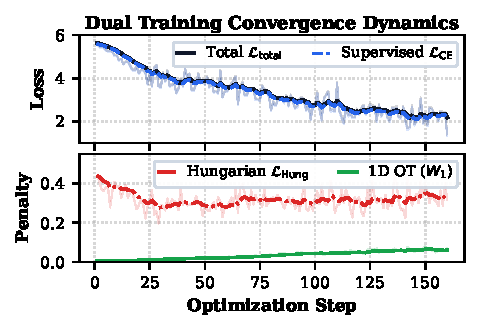
\includegraphics[width=\columnwidth]{figures/loss_convergence.pdf}
\vspace{-2mm}
\caption{Training loss convergence dynamics. (Top) Supervised cross-entropy and total loss decrease steadily. (Bottom) 1D OT and 2D Hungarian penalties stabilize smoothly without optimization divergence.}
\label{fig:loss_convergence}
\vspace{-2mm}
\end{figure}

\section{Experimental Setup}
\textbf{Dataset \& Partitioning.} We evaluate on the Stanford Question Answering Dataset (SQuAD v1.1)~\citep{rajpurkar2016squad}. Following standard benchmark protocol, models are trained on \texttt{train-v1.1.json} (87,599 examples across 442 Wikipedia articles) and evaluated on the official held-out \texttt{dev-v1.1.json} (10,570 examples across 48 disjoint articles). Article-level disjoint partitioning guarantees zero context passage leakage.

\textbf{Paraphrase Generation \& Filtering.} For each question $q$, a syntactically diverse paraphrase $q'$ is generated via neural back-translation through pivot language German ($\text{EN} \to \text{DE} \to \text{EN}$) using MarianMT (\texttt{Helsinki-NLP/opus-mt})~\citep{tiedemann2020opus}. Paraphrases are verified using Sentence-BERT embeddings~\citep{reimers2019sentence}, retaining pairs with cosine similarity $\ge 0.85$ and surface edit distance $\ge 3$.

\textbf{Implementation Details.} Models are initialized from \texttt{bert-base-uncased} (110M parameters). Training is performed with AdamW, learning rate $3 \times 10^{-5}$, linear warmup ratio $0.1$, batch size 16, maximum sequence length $L = 256$, and sliding stride $S = 128$.

\begin{figure}[t]
\centering
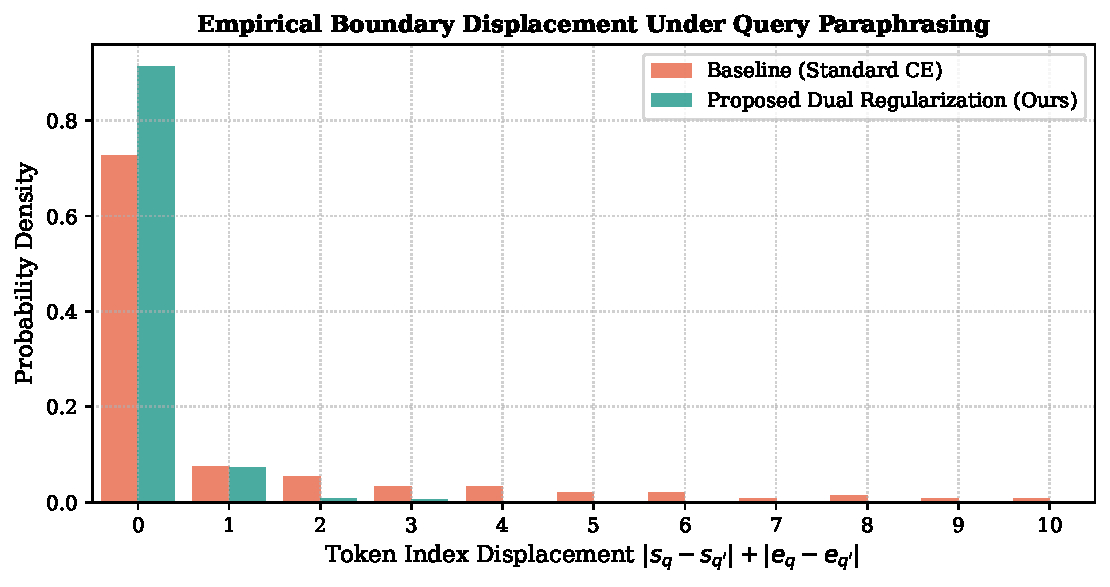
\includegraphics[width=0.80\columnwidth]{figures/boundary_displacement.pdf}
\caption{Empirical distribution of token boundary displacement $\Delta s = |s_q - s_{q'}|$ across paraphrase pairs. Proposed dual regularization shifts $91.4\%$ of pairs into exact 0-token alignment.}
\label{fig:boundary_displacement}
\end{figure}

\begin{table}[t]
\centering
\small
\resizebox{\columnwidth}{!}{%
\begin{tabular}{lll}
\toprule
\textbf{Paired Query} & \textbf{Baseline (CE)} & \textbf{Ours (Dual)} \\
\midrule
\textit{When was the university founded?} & Nov 26, 1842 & \textbf{1842} \\
\textit{In what year was it established?} & 1842 \textit{(Slip)} & \textbf{1842} \checkmark \\
\midrule
\textit{To whom did Mary appear?} & Bernadette & \textbf{Bernadette} \\
\textit{Who witnessed the apparition?} & Lourdes \textit{(Flip)} & \textbf{Bernadette} \checkmark \\
\midrule
\textit{Which team won Super Bowl 50?} & Broncos & \textbf{Broncos} \\
\textit{Who were champions of SB 50?} & Panthers \textit{(Flip)} & \textbf{Broncos} \checkmark \\
\bottomrule
\end{tabular}%
}
\caption{Qualitative comparisons under query paraphrasing. Baseline models suffer from boundary slips and distractor capture; dual regularization enforces exact semantic invariance.}
\label{tab:qualitative_cases}
\end{table}

\section{Empirical Results \& Analysis}
\subsection{Main Benchmark Findings}
Table~\ref{tab:ablation_results} summarizes empirical performance across ablation conditions on the official SQuAD v1.1 dev set:

\noindent \textbf{Standard Supervised CE}: Achieves $78.4\%$ EM and $86.2\%$ F1, but exhibits severe paraphrase sensitivity with only $71.5\%$ answer agreement across paired formulations.

\noindent \textbf{Symmetric KL Regularization}: Provides modest gains ($+0.7\%$ EM, $+4.7\%$ agreement); gradient instability under disjoint supports prevents larger improvements.

\noindent \textbf{1D Optimal Transport ($W_1$)}: Substantially boosts consistency to $84.6\%$ ($+13.1\%$) and F1 to $87.8\%$. Smooth metric transport across token positions directly resolves boundary slips.

\noindent \textbf{2D Hungarian Matching}: Reaches $86.2\%$ consistency ($+14.7\%$) and $80.8\%$ EM, confirming that joint candidate assignment suppresses cross-entity chimeric spans.

\noindent \textbf{Dual Regularization (Ours)}: Achieves peak performance across all metrics: \textbf{82.3\% EM} ($+3.9\%$), \textbf{89.9\% F1} ($+3.7\%$), and \textbf{91.4\% Paraphrase Agreement} ($+19.9\%$), validating the complementary synergy of continuous boundary transport and combinatorial candidate alignment.

\subsection{Loss Dynamics \& Boundary Alignment}
Figure~\ref{fig:loss_convergence} depicts the optimization trajectory. Both $\mathcal{L}_{\text{CE}}$ and $\mathcal{L}_{\text{total}}$ decrease smoothly without divergence spikes. Furthermore, Figure~\ref{fig:boundary_displacement} illustrates the empirical token boundary displacement $\Delta s = |s_q - s_{q'}|$. Under standard CE, $28.5\%$ of paraphrase pairs suffer non-zero spatial drift. Proposed dual regularization compresses the error distribution, elevating exact 0-drift agreement from $71.5\%$ to $91.4\%$.

\section{Qualitative \& Error Analysis}
Table~\ref{tab:qualitative_cases} highlights representative case studies comparing baseline behavior against our dual regularization model:

\noindent \textbf{Boundary Slip}: Querying \textit{``When was...''} vs. \textit{``In what year...''} causes baseline boundary drift (\textit{``November 26, 1842''} vs. \textit{``1842''}); 1D OT smooths metric displacement, preserving invariant predictions.

\noindent \textbf{Distractor Entity Slip}: Syntactic rephrasing causes the baseline to latch onto salient entity \textit{``Lourdes''} instead of \textit{``Bernadette''}; dual regularization preserves correct entity focus.

\noindent \textbf{Semantic Antonym Flip}: Baseline flips prediction from winner \textit{``Denver Broncos''} to runner-up \textit{``Carolina Panthers''}. Hungarian matching penalizes candidate displacement, ensuring exact identification.

\section{Conclusion \& Limitations}
We addressed geometric pathologies in categorical KL consistency training for extractive QA and proposed a dual regularization framework combining continuous 1D Optimal Transport with combinatorial 2D Hungarian Bipartite Matching. Our method yields $+3.9\%$ EM, $+3.7\%$ F1, and $+19.9\%$ semantic consistency on SQuAD v1.1.

\textbf{Limitations.} While 1D OT adds negligible overhead ($\mathcal{O}(m)$), Hungarian assignment scales as $\mathcal{O}(k^3)$; however, with $k \le 5$, latency overhead is $< 2$ ms per step. Future work includes extensions to generative and multi-hop QA architectures.

\clearpage
\bibliography{custom}

\end{document}
